\documentclass[a4paper,10pt,twocolumn]{article}


\usepackage[utf8]{inputenc} % Support for UTF-8 encoding
\usepackage[T1]{fontenc}    % Better font rendering
\usepackage{graphicx}       % For including images
\usepackage{tabularx}
\usepackage[colorlinks=true, linkcolor=black, citecolor=black, filecolor=black, urlcolor=blue]{hyperref}
\usepackage{geometry}       % To adjust margins
\geometry{margin=2.5cm}
\usepackage{titlesec}       % For custom section headings
\usepackage{fancyhdr}       % For header and footer customization
\usepackage{natbib}         % For in-text citations (Harvard style)
\usepackage{lmodern}        % Improved font quality
\usepackage{setspace}       % For adjusting line spacing
\usepackage{ragged2e}       % Fix justification issues
\usepackage[protrusion=true,expansion=true]{microtype} % Better text spacing
\usepackage{longtable}
\usepackage{amsmath}        % Provides \numberwithin
\usepackage{makecell}
\usepackage{enumitem}
\numberwithin{figure}{section}
\numberwithin{table}{section}
\renewcommand{\thefigure}{\thesection-\arabic{figure}}

% \usepackage{parskip}   % This removes indentation and adds spacing between paragraphs
\setlength{\parindent}{1em}  % First-line indentation for paragraphs
\setlength{\parskip}{0pt}     % No extra space between paragraphs

% ---- Fix fancyhdr warning: set proper headheight ----
\setlength{\headheight}{14.5pt}

% ---- Header settings ----
\pagestyle{fancy}
\fancyhf{}
\rhead{KTH}
\cfoot{\thepage}

% ---- SUB SBUB no stretch settings ----
\usepackage{xspace} % Ensures spacing works correctly
\titleformat{\subsubsection}
  {\normalfont\normalsize\bfseries} % Normal font size, bold
  {\thesubsubsection} % Keep numbering
  {1em} % Indentation before text
  {\raggedright} % Prevent text stretching

\titlespacing{\subsubsection}{0pt}{0pt}{0pt} % Remove extra spacing


% --------------------------------------------------------------------------------------------------------------------------------------------


\begin{document}


% ---- Suppress page numbering on title page to avoid duplicate "page.1" link ----
\clearpage
\pagenumbering{gobble}  % Removes the page number but avoids identifier conflicts

\setlength{\headheight}{14.5pt}
% ---- Title Page ----
\begin{titlepage}
    \centering
    
\includegraphics[width=0.2\textwidth]{kthLogga.png}\\[1cm]
    {\large BACHELOR'S THESIS IN COMPUTER SCIENCE AND INDUSTRIAL ECONOMICS}\\[0.5cm]
    {\large UNDERGRADUATE LEVEL 15 CREDITS}\\[3cm]
    {\Huge \textbf{A Comparative Evaluation of Open-Source Digital Asset Management Systems}}\\[0.5cm]
    
    {\Large Exploring Organizational and Marketing Criteria for Process and Marketing Innovation in SMEs}\\[1cm]
    \vfill
    {\Large \textbf{ELLA KARLSSON}}\\[1cm]
    \vfill
    {\large School of Industrial Engineering and Management}\\
    {\large Royal Institute of Technology (KTH)}\\
\end{titlepage}

% --------------------------------------------------------------------------------------------------------------------------------------------
% The Influence of Neural
% Network-based Image
% Enhancements on Object
% Detection

% ===== Section 1: abstract och sammanfattning... =====
\newpage
\pagenumbering{arabic}
\onecolumn
\phantomsection 
\section*{Abstract}
\addcontentsline{toc}{section}{Abstract}

\citep{author2025}

•	What is the topic area? (optional) Introduces the subject area for the project.
•	Short problem statement
•	Why was this problem worth a Master’s thesis project? (i.e., why is the problem both significant and of a suitable degree of difficulty for a Master’s thesis project? Why has no one else solved it yet?)
•	How did you solve the problem? What was your method/insight?
•	Results/Conclusions/Consequences/Impact: What are your key results/conclusions? What will others do based upon your results? What can be done now that you have finished - that could not be done before your thesis project was completed?

\vspace{0.3cm} 
\textbf{Keywords:} 
    
Digital Asset Management (DAM), Version Control, Metadata Management, Access Control, SMEs, Workflow Optimization

\phantomsection 
\section*{Sammanfattning}
\addcontentsline{toc}{section}{Sammanfattning}

\vspace{0.3cm} 
\textbf{Nyckelord:} 
\newpage

\phantomsection 
\section*{Acknowledgments}
\addcontentsline{toc}{section}{Acknowledgments}
I would like to thank xxxx for having yyyy.

% ---- Table of Contents, list of tables, figures ----
\newpage
\phantomsection 
\onecolumn
\tableofcontents
\newpage

\newpage
\phantomsection 
\addcontentsline{toc}{section}{List of Figures}
\listoffigures
\newpage
\phantomsection 
\addcontentsline{toc}{section}{List of Tables}
\listoftables

% ---- List of Acronyms and Abbreviations ----
\newpage
\phantomsection
\addcontentsline{toc}{section}{List of Acronyms and Abbreviations}
\section*{List of Acronyms and Abbreviations}
\vspace{0.2cm} % Add some space to align table with the heading

\renewcommand{\arraystretch}{1.2} % Adjust row height for readability
\begin{flushleft} % Align the table properly with the heading
\begin{longtable}{p{5cm} p{12cm}} % Adjust column width for proper alignment
    
    AI   & Artificial Intelligence \\
    DAM  & Digital Asset Management \\
    DSR  & Design Science Research \\
    DT   & Digital Transformation \\
    ERP  & Enterprise Resource Planning \\
    IT   & Information Technology \\
    ML   & Machine Learning \\
    MCS  & Management Control Systems \\
    MDM  & Metadata Management \\
    RBAC & Role-based access control \\
    RBV  & Resource-Based View \\
    SME  & Small and Medium-sized Enterprises \\
    UX   & User Experience \\
    VRIN & Valuable, Rare, Inimitable, Non-substitutable \\
    YOLO & You Only Look Once \\
    
\end{longtable}
\end{flushleft}


% --------------------------------------------------------------------------------------------------------------------------------------------

% ---- Switch Back to Two-Column Layout for Main Content ----
\twocolumn
\flushbottom % ÄNDR


% ===== Apply Spacing Fixes =====
% \RaggedRight   % Disable full justification to avoid stretched text
\sloppy        % Allow better text breaking to prevent large spaces
\hyphenpenalty=500
\tolerance=1000


% ===== Section 2: Introduction =====

\section{Introduction}

To be added 
state-of-the-art one-stage object detection algorithm 
renowned for its efficiency and simplicity
% This chapter describes the specific problem that this thesis addresses, the context of the problem,
% the goals of this thesis project, and outlines the structure of the thesis.
% Give a general introduction to the area. (Remember to use appropriate references in this and all
% other sections.)

\subsection{Background}
Digital Asset Management (DAM) emerged in the late 1990s as organizations began grappling 
with the rapid increase in digital content \citep{krogh2009}. Early DAM systems were primarily on-premises 
solutions designed to store and manage assets such as images, videos, and documents. 
In the early 2000s, these systems transitioned to cloud-based platforms, offering 
improved scalability and accessibility \citep{mccain2021}.

More recently, the integration of Artificial Intelligence (AI) and machine learning (ML) has transformed 
DAM by automating key processes like image tagging, sorting, and categorization. Advanced computer 
vision techniques now enable systems to analyze and tag images automatically, 
reducing manual effort and increasing accuracy \citep{MINGfANG}.

% \begin{figure}[htbp]
%     \centering
%     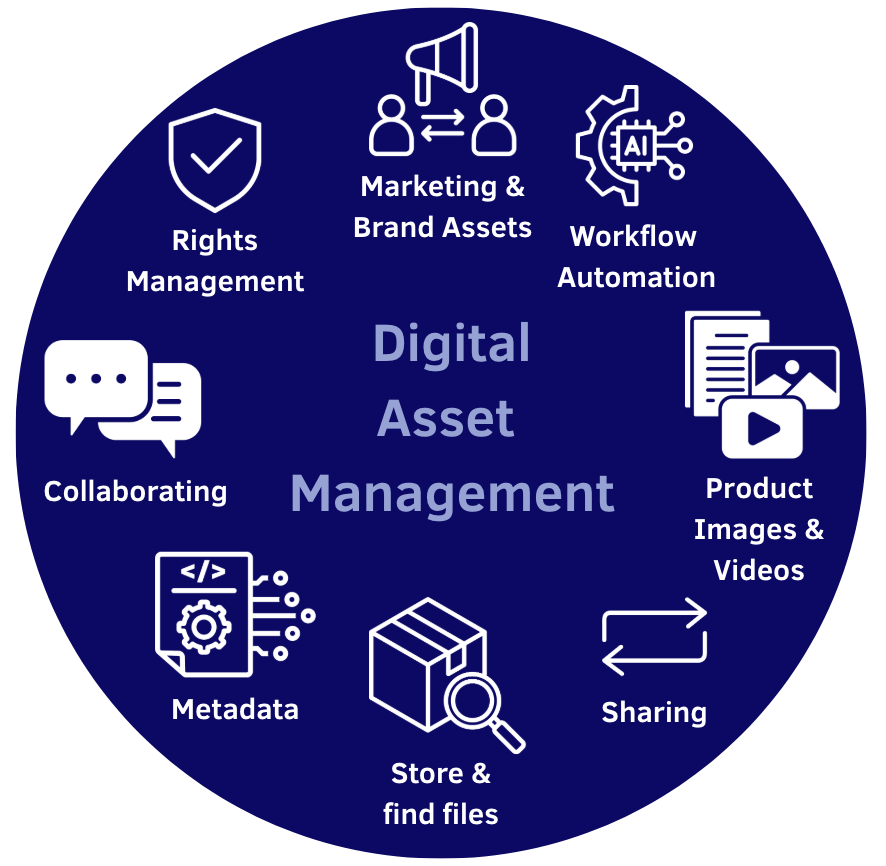
\includegraphics[width=0.95\linewidth]{DAMC.png}  % Replace with actual image file
%     \caption{Illustrating components of a modern DAM system}
%     \label{fig:DAMC}  
% \end{figure}

% Present the background for the area. Set the context for your project – so that your reader can
% understand both your project and this thesis. (Give detailed background information in Chapter 2 -
% together with related work.)
% Sometimes it is useful to insert a system diagram here so that the reader knows what are the
% different elements and their relationship to each other. This also introduces the names/terms/…
% that you are going to use throughout your thesis (be consistent). This figure will also help you later
% delimit what you are going to do and what others have done or will do.
% As one can find in RFC 1235 [1] multicast is useful for xxxx

\subsection{Problem}
As bespoke manufacturers scale, managing digital assets—spanning product imagery, design renderings,
and technical specifications—becomes essential for brand consistency and operational efficiency.
However, most DAM solutions, especially open-source systems, lack the necessary automation, 
posing adoption and maintenance challenges for small and medium-sized enterprises (SMEs) with limited IT infrastructure. 
Wu et al. studied automated metadata annotation for cultural heritage and found that AI-generated 
captions often oversimplify context, such as describing a medieval knight merely as a “man on a horse” \citep{MINGfANG} 
This reflects similar challenges in design-driven manufacturing, where internal product terminology and industry-specific 
references require more precise and context-aware interpretation.

A core function of DAM is image tagging, sorting, and categorization, directly influencing asset 
retrievability and structural organization. Although AI has been integrated into some DAM solutions,
 these implementations typically rely on large pre-trained models that offer broad object classification 
 rather than domain-specific tagging and vocabulary. Recent advancements in computer vision, 
 particularly through algorithms such as YOLO (You Only Look Once), 
offer an opportunity to overcome these limitations. However, deploying a YOLO-powered system in this domain
 requires adapting the model to the specific features and vocabulary of the manufacturing sector. Rather than
  training a model from scratch—a process that demands extensive annotated data and computational resources—a 
  more feasible approach is to fine-tune a pre-trained model using company-specific data. 


\subsection{Purpose}
% State the purpose of your thesis and the purpose of your degree project.
% Describe who benefits and how they benefit if you achieve your goals. Include anticipated
% ethical, sustainability, social issues, etc. related to your project. (Return to these in your reflections
% in Section 6.4.) /
This study focuses on the metadata generation stage of Digital Asset Management 
(DAM), particularly automated image tagging using deep learning models.

The primary aim of this thesis is to assess the feasibility and impact of a YOLO-powered DAM system 
that has been fine-tuned on company-specific data to address the unique needs of premium manufacturing SMEs. 
The research will benchmark the performance of this fine-tuned system against a conventional open-source DAM 
platform (ResourceSpace), focusing on improvements in asset categorization accuracy
and retrieval efficiency. 

\vspace{0.3cm}
\subsubsection{Technical Research questions}
\vspace{0.3cm}

\begin{enumerate}[label=(\alph*)]
    \item To what extent does fine-tuning YOLOv11 and 
    Faster R-CNN on company-specific manufacturing data 
    improve object detection accuracy compared to a 
    baseline model, in terms of precision, recall, 
    and inference speed?

    \item What are the trade-offs between YOLOv11 and 
    Faster R-CNN in terms of tagging quality, computational
    cost, and integration complexity within a DAM workflow?
    
    \item How do differences in model performance impact the 
    usefulness of metadata for downstream tasks such as asset 
    retrieval and categorization?

\end{enumerate}

\subsubsection{Business Research questions}
\vspace{0.3cm}
Technological advancements alone do not guarantee successful integration. To complement this,
the business perspective assesses the organizational and strategic impact after selecting the preferred DAM system. Specifically:

\begin{enumerate}[label=(\alph*), resume]
    \item What organizational and process changes are 
    required to integrate AI-based image tagging into a manufacturing 
    SME, and how do these changes affect knowledge structuring and 
    internal workflows?
    
    \item What barriers emerge during implementation, and how are they
    influenced by the organization’s flexibility, strategic priorities, 
    and project-based work culture?

    \item How does improved metadata generation contribute to long-term 
    business value, such as brand consistency, operational scalability, and process innovation?
    
\end{enumerate}   

\subsubsection{Societal Impact}
\vspace{0.2cm}
Digital transformation has a significant impact on SMEs.
These companies account for approximately 60\% of total turnover and value-added 
contributions in Sweden’s private sector, employing around 65\% of the 
workforce \citep{tillvaxtverket2021}.
The adoption of DAM systems is an integral part of this transformation, 
improving operational efficiency and reducing manual work,
which contributes to broader economic growth. A cost-benefit analysis of 319 SMEs 
found that digital transformation enhances organizational resilience, reduces 
operational costs, and improves long-term scalability \citep{teng2022}.

\vspace{0.3cm}
The stakeholders of this project?

This study is structured around a systematic process 
encompassing data collection, annotation, model fine-tuning, and testing. 
These phases represent essential steps that an SME would need to undertake 
if they were to implement a similar AI-based solution. 
By addressing both the positive impacts and the possible challenges, the aim is to
to show if the benefits of adopting this solution
justify the necessary investments and efforts.
The project’s outcomes are expected to contribute to 
academic knowledge in the field of AI-powered asset management, 
fostering further innovation. 

\vspace{0.3cm}
\subsubsection{Ethical considerations}
\vspace{0.2cm}
Ethically, the project will investigate issues related to data privacy, 
 transparency, and bias, which are critical in ensuring that 
automated systems operate fairly and without unintended consequences. 
These concerns are highlighted in the literature on AI ethics, which emphasizes 
the need for clear guidelines to mitigate risks associated with autonomous decision-making\citep{jobin2019global}.

\vspace{0.3cm}
\subsubsection{Sustainability, and social considerations}
\begin{figure}[htbp]
    \centering
    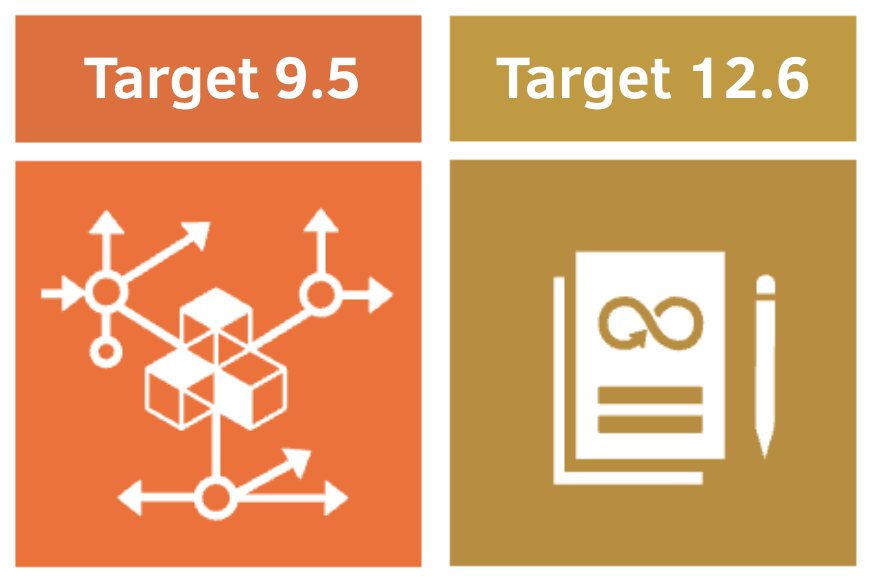
\includegraphics[width=0.48\linewidth]{targets.png}  % Replace with actual image file
    \caption{Sustainable Development Target 9.5 and 12.6}
    \label{fig:targets}  
\end{figure}

From a sustainability perspective, this research contributes to the United Nations Sustainable 
Development Goals (SDGs), specifically SDG 9, Industry, Innovation, and Infrastructure, and SDG 12, 
Responsible Consumption and Production, \citep{UN2030Agenda}. 
In relation to SDG 9, and more precisely 
target 9.5 as seen in Figure \ref{fig:targets}, the project seeks to enhance scientific 
research and upgrade the technological capabilities
 within industrial sectors. Similarly, under SDG 12 target 12.6 also shown in \ref{fig:targets}, 
 this project supports sustainable business practices by optimizing digital 
asset management. By enhancing asset categorization and retrieval, the system makes it easier 
for companies to track and store metrics. This dual focus ensures that the technological advancements 
proposed are not only efficient and innovative but also ethically sound and socially beneficial.

\vspace{0.3cm}
Further reflection will be revisited in Section 6.4.



\subsection{Goals}
% State the goal/goals of this degree project.
% The goal of this project is XXX. This has been divided into the following three sub-goals:
% 1. Subgoal \#1
% 2. Subgoal \#2
% 3. Subgoal \#3
% In addition to presenting the goal(s), you might also state what the deliverables and results of
% the project are.

% Note that in the literature study and even the alpha draft, 
% these are your expected goals, deliverables, and results – which may change over the course 
% of the project – hence you will revise this in the final report to describe what you actually 
% achieved, delivered, and produced as results.

The primary goal is evaluating the feasibility of a YOLO-powered DAM
system that has been fine-tuned using company-specific data, 
in comparison to the open-source solution ResourceSpace.
To achieve this, the project has been divided into the following three sub-goals:

\begin{enumerate} 
    
    \item \textbf{Dataset Development and Annotation:}
    Develop a robust methodology for collecting a domain-specific dataset that 
    accurately captures the visual and functional nuances of digital assets 
    in premium manufacturing. The annotation process will involve: 
    \begin{itemize} 
        \item Using bounding boxes to precisely delineate asset regions. 
        \item Assigning appropriate class labels using a standardized labeling schema 
        to ensure consistency and relevance to the manufacturing domain. 
    \end{itemize}
    
    This dataset will serve as the foundation for model fine-tuning.

    \item \textbf{Model Fine-Tuning and Optimization:}  
    Fine-tune a pre-trained YOLO model on the annotated dataset. 
    The objective is to enhance the model’s 
    accuracy in tagging, sorting, and categorizing.
    \begin{itemize}
        \item Adjusting hyperparameters and leveraging transfer learning techniques.
        \item Implementing regularization and validation strategies.
    \end{itemize}

    \item \textbf{Performance Benchmarking and Comparative Analysis:}  
    Benchmark the performance of the fine-tuned YOLO-based DAM system against a 
    conventional open-source DAM called ResourceSpace. Evaluation metrics will include:
    \begin{itemize}
        \item Asset categorization accuracy.
        \item Retrieval efficiency.
        \item Overall system usability.
    \end{itemize}
\end{enumerate}

A comparative analysis will be conducted to assess whether the customized 
system offers significant improvements over traditional solutions. 
Resulting in practical recommendations 
and guidelines for manufacturing SMEs 
considering the adoption of AI-powered DAM.


\subsection{Research Methodology}
This research employs a mixed-methods approach to address both the 
technical performance of the system and stakeholder perspectives. 
Mixed-methods research combines quantitative techniques 
(e.g., controlled experiments and statistical analyses) with 
qualitative techniques (e.g., semi-structured interviews and thematic analysis)
to provide a comprehensive evaluation of complex systems \citep{johnson2004mixed}.

Alternative methodologies—such as exclusively quantitative performance evaluations 
or purely qualitative case studies—were considered but ultimately rejected because 
they would not fully capture the multifaceted challenges of deploying an AI-powered 
system in a dynamic industrial environment.

\vspace{0.3cm}
\subsubsection{Design Science Approach}
\vspace{0.3cm}

% Introduce your choice of methodology/methodologies and method/methods – and the reason why
% you chose them. Contrast them with and explain why you did not choose other methodologies or
% methods. (The details of the actual methodology and method you have chosen will be given in
% Chapter 3. Note that in Chapter 3, the focus could be research strategies, data collection, data
% analysis, and quality assurance.)
% In this section you should present your philosophical assumption(s), research method(s), and
% research approach(es).

Grounded in a pragmatic philosophy that emphasizes practical impact and utility, 
this study adopts the design science research (DSR) paradigm. DSR is particularly 
well-suited for technology-driven projects because it promotes the iterative design, 
development, and rigorous evaluation of IT artifacts to solve 
real-world problems \citep{hevner2004design}. In this project, 
the YOLO-powered DAM system represents 
the artifact developed and refined through iteration.

\vspace{0.3cm}
\subsubsection{Quantitative and Qualitative Methods }
\vspace{0.3cm}
Controlled experiments will be conducted to measure key performance 
metrics—such as asset categorization accuracy, retrieval efficiency, 
and overall system usability. Statistical analysis w
ill be used to validate the improvements brought about by model fine-tuning, 
following best practices in empirical research \citep{creswell2014, yin2014case}.
Complementing this, qualitative methods will capture contextual insights and 
stakeholder perspectives. Semi-structured interviews and thematic analysis 
will be employed to understand user experiences and organizational challenges 
associated with implementing the DAM system. 
Moreover, to develop a standardized 
labeling schema for the dataset, a targeted collaboration with a designated 
expert from the company will be undertaken. This focused approach is 
preferred over a large-scale survey. Not all employees interact 
with digital assets and the expert can ensure domain-specific 
terminology is accurately captured and applied consistently during annotation.

\subsection{Delimitations}
% Describe the boundary/limits of your thesis project and what you are explicitly not going to do. This
% will help you bound your efforts – as you have clearly defined what is out of the scope of this
% thesis project. Explain the delimitations. These are all the things that could affect the study if they
% were examined and included in the degree project.
This thesis focuses exclusively on evaluating a YOLO-powered digital asset management 
system for premium manufacturing SMEs. The study is limited to a specific company’s 
environment and a predefined dataset.

The research investigates only the fine-tuning of an existing pre-trained YOLOv11 model. 
Training a model from scratch, which requires vast amounts of data and computational resources, 
is beyond the scope of this project.
Instead of conducting a large-scale survey, the study uses semi-structured interviews with key 
stakeholders—particularly a designated domain expert—to develop a standardized labeling schema. 

This focused approach is chosen because only a few employees directly manage digital assets.
The assessment will concentrate on technical performance indicators such as asset categorization accuracy, 
retrieval efficiency, and overall system usability. Broader issues such as integration with other enterprise systems 
and macroeconomic impacts are beyond the scope of this project.

\subsection{Structure of the thesis}
% Chapter 2 presents relevant background information about xxx. Chapter 3 presents the
% methodology and method used to solve the problem. …
% Exclude the first chapter , references, and appendix/appendices. 

This thesis is organized into the following main chapters, 
excluding the introductory chapter, references, and appendices; 
Chapter 2 provides the necessary background and reviews related work,
 establishing the context for DAM and identifying the key gaps this project addresses. 
 Chapter 3 outlines the methodology—including the design science approach, 
 mixed-methods strategy, data collection, experimental design, and evaluation 
 criteria—used to assess the system. 
 Chapter 4 details the implementation, covering system design, 
 model fine-tuning, dataset development, and the technical setup for testing. 
 Chapter 5 presents the results and analysis, discussing both quantitative 
 metrics and qualitative insights to evaluate whether the project’s goals have been met. 
 Finally, Chapter 6 summarizes the key findings, reflects on the limitations of the study, 
 and outlines potential directions for future work.




% --------------------------------------------------------------------------------------------------------------------------------------------
\newpage
% ===== Section 2: Background =====
\section{Background}
% This chapter provides basic background information about xxx. Additionally, this chapter describes
% xxx. The chapter also describes related work xxxx.
% What does a reader (another x student -- where x is your study line) need to know to understand
% your report?
% What have others already done? (This is the “related work”.) Explain what and how prior work /
% prior research will be applied on or used in the degree project /work (described in this thesis).
% Explain why and what is not used in the degree project and give valid reasons for rejecting the
% work/research.

% When you do your literature study, you should have a nearly complete Chapters 1, 2.

% You may also find it convenient to introduce the 
% future work section into your report early – so that you can 
% put things that you think about but decide not to do now into this section.

% Note that later you can move things between this future work section and what 
% you have done as you may change your mind about w
% hat to do now versus what to put off to future work.

\subsection{\mbox{Artificial Inteligence}}
Artificial Intelligence (AI) is a field of computer science 
that focuses on systems built on algorithms, 
which are formalized sets of instructions that 
process input data to produce outputs \citep{10589380}. 
Machine Learning (ML), a subset of AI, represents a shift away 
from manually encoded rules toward data-driven learning. 
Instead of being explicitly programmed for specific tasks, 
ML models identify patterns in large datasets and 
use statistical techniques to make predictions or classify new data.

\cite{10589380} describe deep learning (DL) as a machine learning 
approach that utilizes multi-layered computational models to 
extract patterns from data at varying levels of abstraction. 
Inspired by the human brain, DL models excel at recognizing 
intricate patterns in large datasets.
\citep{SOORI202354} further eplains that within DL, 
different neural network architectures are designed to process
 specific types of data and perform specialized tasks. 
 One of the most effective architectures for structured, 
 grid-like data—such as images—is 
 the Convolutional Neural Network (CNN). 
 CNNs employ convolutional operations to automatically 
 learn spatial hierarchies of features, allowing them to 
 capture patterns and structures in data with high accuracy. 
 As a result, CNNs have become a cornerstone of computer vision, 
 powering applications in object detection, image classification, 
 and other visual recognition tasks \citep[pp. 326-328]{Goodfellow-et-al-2016}.

\vspace{0.3cm}
\subsubsection{Object Detection}
\vspace{0.3cm}
Object detection involves both the ability to recognize the classes of multiple objects in an image
and determining their positions, whereas image classification assigns a single 
class to the entire image without distinguishing individual objects.

\cite{ZhangLei2025RoMH} outline how DL-based object 
detection methods are primarily divided into two categories: 
two-stage and single-stage networks. 
Two-stage networks, such as Region-Based Convolutional Neural Networks (R-CNNs), 
rely on generating region proposals before classifying and refining object 
locations. In contrast, single-stage networks, such as You Only Look Once (YOLO),
 eliminate this intermediate step by predicting object classes
 and bounding boxes in a single pass. This approach significantly improves 
 detection speed and efficiency. As Zhang et al. (2025) emphasize, 
 single-stage models have become widely adopted in various industries 
 due to their ability to perform real-time object detection accurately.

 \vspace{0.3cm}
\subsubsection{\mbox{Anchor-free detection models}}
\vspace{0.3cm}

A bounding box defines an object's position and size within an image using four coordinates. 
In object detection, it is paired with a class label and a confidence score, indicating both the object's 
category and the model's certainty in its prediction.
These boxes act as ground-truth references in training data, helping models learn to localize objects accurately.
\citep{li2022yolov6}. The prediction represents the 
final output of an object detection model as illustrated in Figure \ref{fig:bounding}.

\begin{figure}[h]
    \centering
    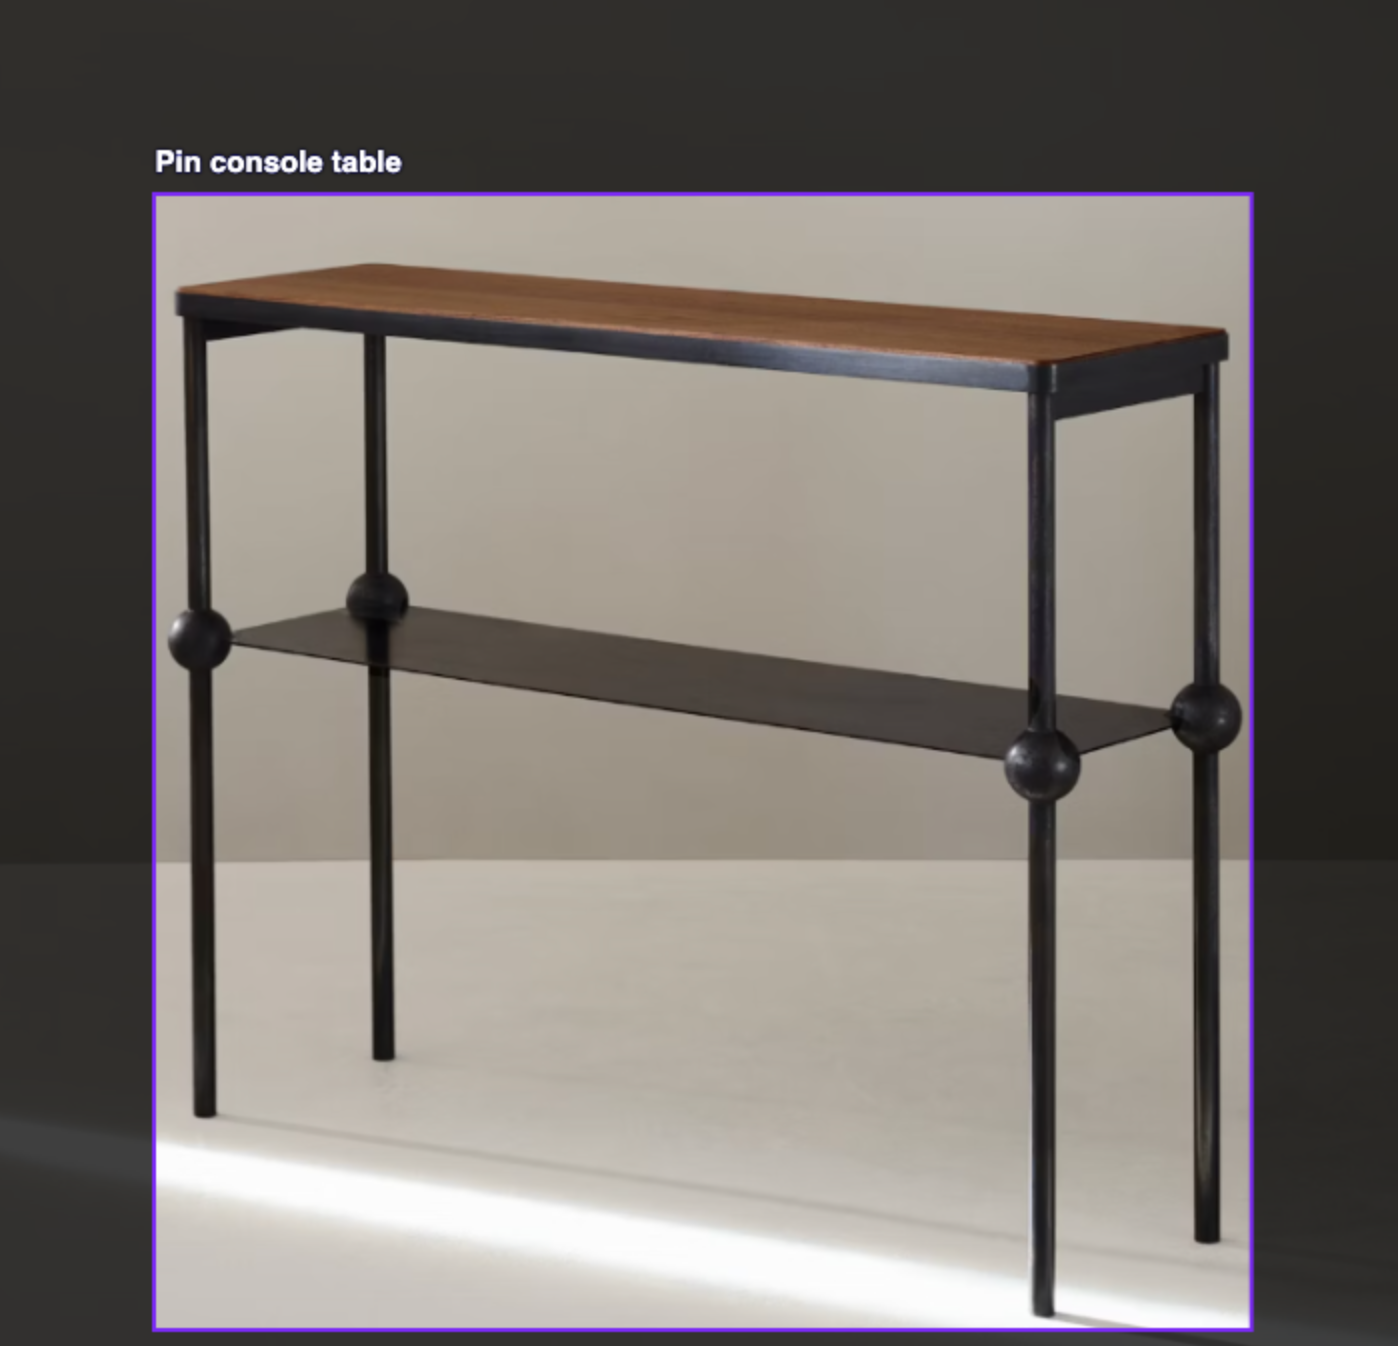
\includegraphics[width=0.7\linewidth]{bounding.png}  % Replace with actual image file
    \caption{Bounding box for table with legs.}
    \label{fig:bounding}  
\end{figure}


\cite{vina2024yolo11} describes the shift from anchor-based to anchor-free
object detection as a major advancement in the field. Traditional anchor-based 
detectors, such as YOLOv4 and its predecessors in Table 
\ref{tab:yolo_versions}, rely on predefined anchor 
boxes—fixed-size reference shapes placed across an image at different aspect 
ratios—to estimate object locations. The model does not predict bounding boxes 
directly but instead modifies the closest anchor to better fit detected objects.
Anchor-free models simplify detection and improve speed—critical for 
real-time tasks like autonomous driving and surveillance. Their
 key-point-based approach enhances flexibility, making them better at detecting small,
  irregular, or occluded objects, especially in cluttered environments 
  where anchor-based methods struggle \citep{wang2024yolov9}.

\vspace{0.3cm}
\subsection{{The Architecture of a Convolutional Neural Network}}
\vspace{0.3cm}

\cite{prince2023understanding} highlights three key characteristics of
digital images that necessitate the use of specialized model architectures. 
First, images are inherently high-dimensional. For instance, a standard 224×224 
pixel image with three color channels (RGB) results in over 150,000 input values. 
Processing such a large number of inputs with fully connected neural networks would 
require an impractically high number of parameters. Second, there is a strong correlation 
between neighboring pixels, as local regions often form meaningful patterns and structures. 
Lastly, images tend to be robust to small spatial shifts—their content remains recognizable 
even when objects within them are slightly moved. For instance, if a chair appears slightly 
to the left or right in different images, we still recognize it as the same object. 
However, a fully connected model would need to learn how to identify the chair in every 
possible position from scratch. CNNs such as YOLO and 
Faster R-CNN avoid this problem by using filters that can detect 
patterns no matter where they appear in the image. This makes them far more parameter-efficient and 
better suited for visual tasks like object detection \citep{prince2023understanding}.

At a fundamental level, CNNs process input through sequential stages, 
using convolution to detect spacial features, pooling to 
reduce dimensionality, and activation functions to 
introduce non-linearity \cite{10589380TEST}.
Spatial features can be textures, lines and color variations in the input. 
With effective training, the network learns to recognize 
these attributes regardless of their location within an image \citep[Chapter~2]{VerdhanVaibhav2021CVUD}.

\vspace{0.3cm}
\subsubsection{The Convolutional Operation}
\vspace{0.3cm}

CNNs extract features from images by applying an operation known as convolution \cite[p.~170]{prince2023understanding}. Convolution involves sliding a learnable weight matrix, referred to as a kernel or filter, across the input. At each position, the kernel computes a weighted sum over a local neighborhood of the image, making it possible to detect spatial patterns. Figure~\ref{fig:3D} illustrates this concept. In practice, one often pads the input with zeros (padding) so that the kernel can be applied near image borders without reducing spatial dimensions. Another key hyperparameter is the stride, which specifies how far the kernel moves at each step \cite[p.~165]{prince2023understanding}

\begin{figure}[htbp]
    \centering
    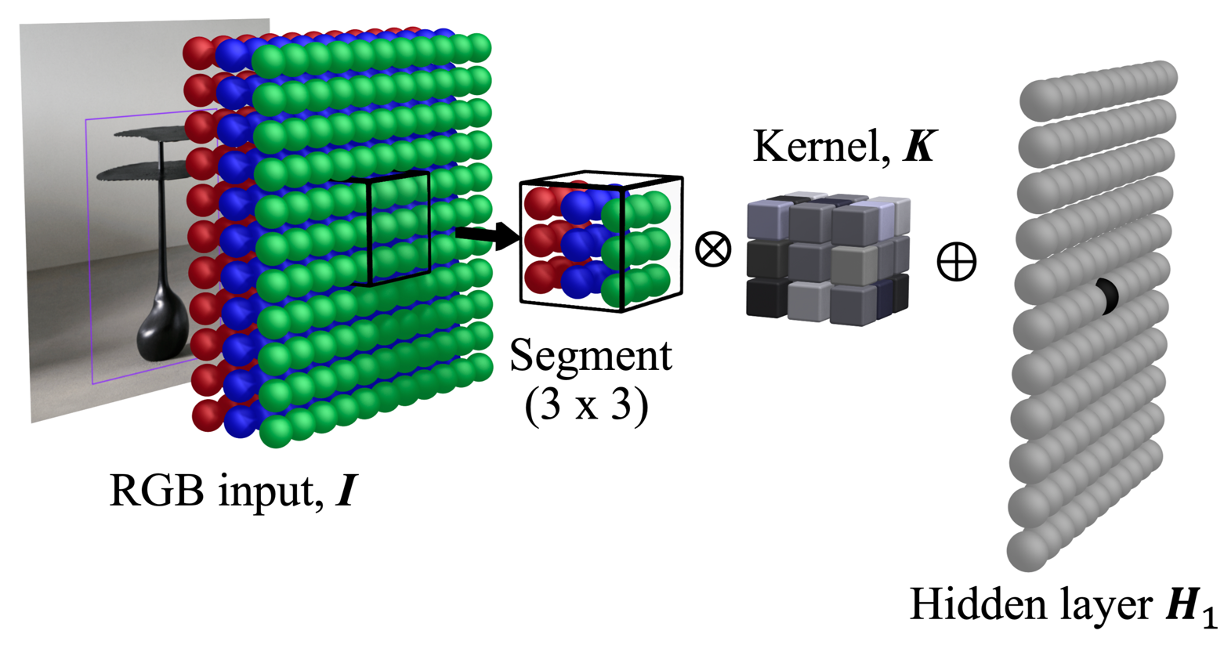
\includegraphics[width=1\linewidth]{3D.png} 
    \caption{A simplified 2D convolution applied to an RGB image (adapted from \citep{prince2023understanding}).}
    \label{fig:3D}  
\end{figure}

Let \(I\) be the input image, structured as three channels (red, green, and blue). Consider a \(3 \times 3 \times 3\) kernel. 
At each spatial position, element-wise multiplication is performed between the kernel weights 
and a \(3 \times 3\) segment from each of the three channels. The products are summed together and then combined with a bias term, producing a pre-activation value that is typically passed through a non-linear function such as ReLU. By shifting the kernel step by step over the height and width of the image, one obtains a two-dimensional feature map. To produce multiple output channels, different kernels run in parallel. Each filter generates its own 2D feature map, and stacking these maps forms a three-dimensional activation tensor, often written as \(H_{1}\).
Equation~\eqref{eq:conv_rgb} demonstrates how the output at position \((i,j)\) can be computed for an RGB input and a \(3 \times 3\) kernel:

\begin{equation}
    \label{eq:conv_rgb}
    \resizebox{0.9\columnwidth}{!}{%
    \(
    \displaystyle
    h_{ij} = a \Bigl(
    b + \sum\limits_{c=1}^{3}
             \sum\limits_{m=1}^{3}
             \sum\limits_{n=1}^{3}
    I_{c,\,i+m-2,\,j+n-2} \cdot K_{c,\,m,\,n}
    \Bigr)
    \)
    }
    \end{equation}
    
    
where \(I_{c,\,i,j}\) denotes the pixel value from channel \(c\) at position \((i,j)\), \(K_{c,\,m,n}\) is the kernel weight for channel \(c\) at offset \((m,n)\), \(b\) is a learnable bias term, and \(a(\cdot)\) represents the chosen activation function
\cite[p.~170]{prince2023understanding}.

\vspace{0.3cm}
\subsubsection{The Pooling Operation}
\vspace{0.3cm}
Pooling is a downsampling operation in CNNs that reduces the spatial dimensions of feature maps while preserving essential features. 
This improves computational efficiency and makes the network less sensitive to small spatial shifts. 
The most common method, max pooling, slides a fixed-size window over the 
feature map and retains only the maximum value in each region as seen in Figure~\ref{fig:pooling} \cite[p.~163]{prince2023understanding}. 

\begin{figure}[htbp]
    \centering
    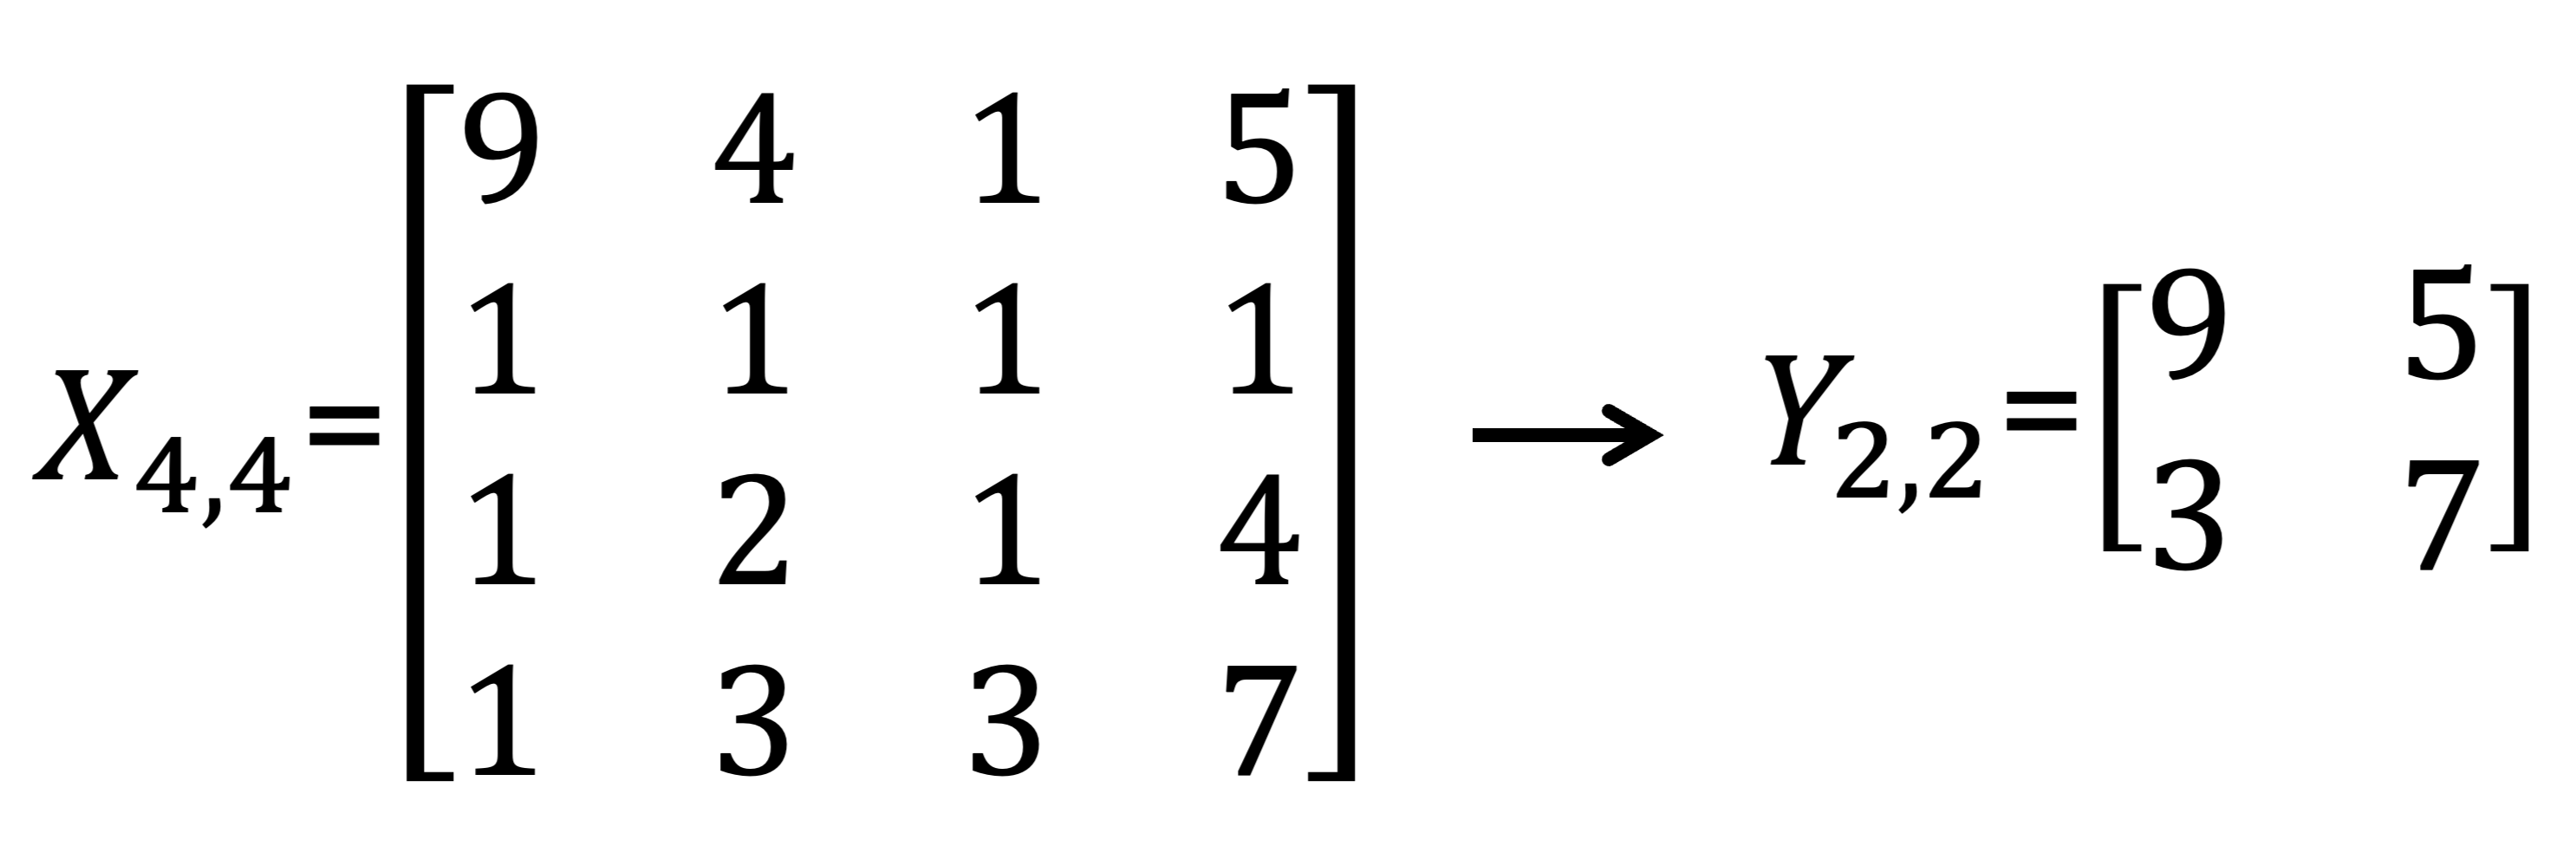
\includegraphics[width=0.6\linewidth]{pooling.png} 
    \caption{Max pooling applied to a \(4 \times 4\) matrix \(X\) resulting in a \(2 \times 2\) matrix \(Y\).}
    \label{fig:pooling}  
\end{figure}

The latest YOLO models developed by \cite{ultralytics2025} extend this concept with the SPPF (Spatial Pyramid Pooling Fast) block, which increases the receptive field through repeated pooling. Figure~\ref{fig:Arc} shows its placement in the Neck in the architecture. The operation is defined as:

\begin{equation} 
    \label{eq:sppf} \mathrm{SPPF} = \mathrm{Conv}_{1 \times 1} \left( \mathrm{Concat}(X,\ P_1,\ P_2,\ P_3) \right) \end{equation}
    
    \noindent
where \( X \) is the input feature map, first passed through a \( 1 \times 1 \) convolution to reduce channel dimensions. \( P_1 = \mathrm{MaxPool}_{5 \times 5}(X) \), \( P_2 = \mathrm{MaxPool}_{5 \times 5}(P_1) \), 
and \( P_3 = \mathrm{MaxPool}_{5 \times 5}(P_2) \). All outputs \( (X, P_1, P_2, P_3) \) are concatenated along the channel 
dimension and passed through a second \( 1 \times 1 \) convolution. 
This design allows the model to capture multi-scale contextual information from 
increasingly larger regions while maintaining spatial resolution, 
which improves object detection performance, especially for small or 
partially occluded objects \citep{ultralytics2025}.

\vspace{0.3cm}
\subsubsection{Activation Functions}
\vspace{0.3cm}

The Ultralytics YOLO architecture by \cite{ultralytics2025} primarily uses the Sigmoid Linear Unit (SiLU), 
also known as \textit{Swish}, as its default activation function. It is defined as
\begin{equation}
\text{SiLU}(x) = x \cdot \sigma(x) = \frac{x}{1 + e^{-x}},
\label{eq:silu}
\end{equation}
where \(\sigma(x)\) represents the sigmoid function. SiLU in Equation~\eqref{eq:silu} offers a smooth non-linearity that helps the model train more efficiently and maintain stronger gradient signals in deep layers.

A simpler alternative, ReLU (Rectified Linear Unit), in Equation~\eqref{eq:relu},
\begin{equation}
\label{eq:relu}
\text{ReLU}(x) = \max(0, x).
\end{equation}
is used in certain parts of the network that benefit from faster computation and sparser activations.
Additionally, some layers omit activations altogether to maintain strictly linear connections.
This is sometimes useful in residual paths or when merging feature maps. 
However, SiLU remains the primary activation due to its observed 
advantages in training stability and overall performance \citep{ultralytics2025}.

\vspace{0.3cm}
\subsubsection{Structural Components of the YOLO Architecture}
\vspace{0.3cm}

The three-part YOLO structure consists of Backbone, Neck, and Head—as shown in Figure \ref{fig:Arc}.
The Backbone extracts features using 
convolutional layers and downsampling, generating hierarchical feature maps.
The Neck refines these features through the SPPF block for multi-scale detection 
and the C2PSA module to enhance the recognition of occluded objects. 
Upsampling and feature concatenation further improve resolution and information 
retention. Finally, the Head produces the model’s output, predicting class probabilities 
and bounding boxes across three detection layers (small, medium and large), 
each specialized for different object sizes \citep{hidayatullah2025yolov8yolo11comprehensivearchitecture}.

\begin{figure}[h]
    \centering
    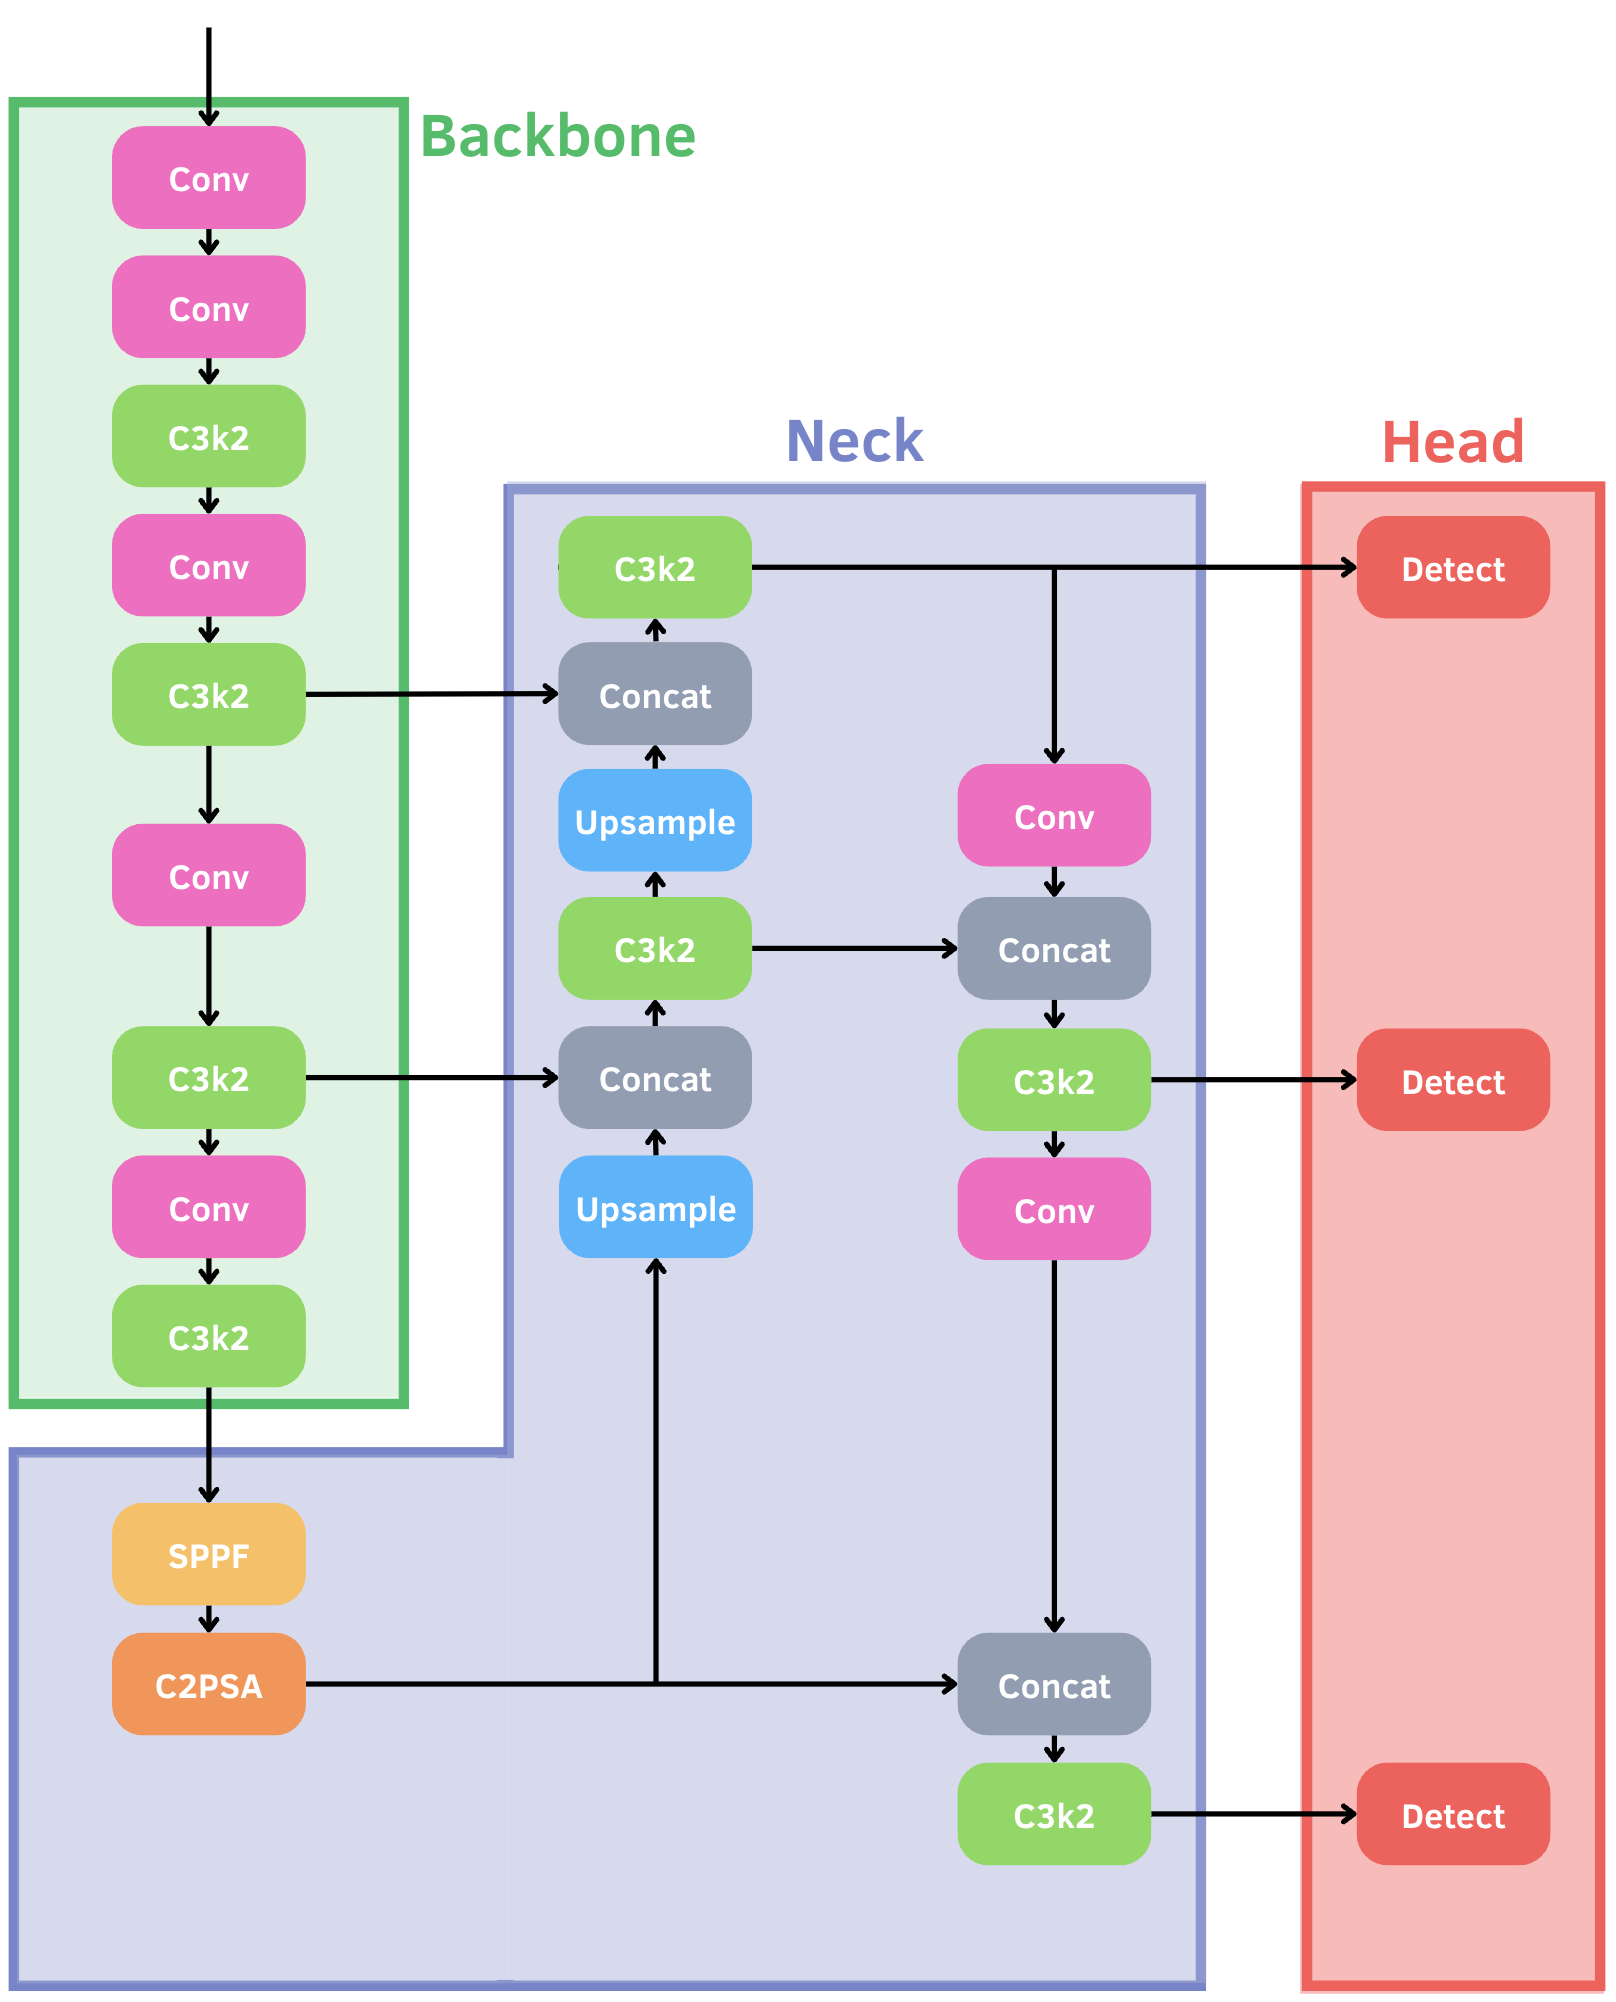
\includegraphics[width=1\linewidth]{YOLOARC.png}  % Replace with actual image file
    \caption{The architecture of YOLOv11, illustrating its three main components: Backbone, Neck, and Head (adapted from \citep{hidayatullah2025yolov8yolo11comprehensivearchitecture}).}
    \label{fig:Arc}  
\end{figure}

The C3k2 module, used in both the Backbone and Neck (Figure \ref{fig:Arc}), 
acts like a compact feature extractor. It splits the input in half: 
one part flows through unchanged, while the other is processed by a stack 
of C3k blocks—convolutions with varied kernel sizes to capture both 
fine and coarse spatial patterns. The two paths are merged and 
compressed through a $1 \times 1$ convolution \citep{hidayatullah2025yolov8yolo11comprehensivearchitecture}.

The C2PSA (Cross-Stage Partial with Position-Sensitive Attention) module following after the SPPF block in Figure \ref{fig:Arc} extends the Cross-Stage Partial (CSP) design with a more expressive attention mechanism known as 
Position-Sensitive Attention (PSA).
While C3k2 in captures features through varied convolution kernels, 
C2PSA uses attention to focus on relevant spatial patterns—especially 
useful for detecting large objects at low resolutions \citep{ultralytics2025}.

Upsampling increases the spatial resolution of feature maps to restore details lost during downsampling. YOLO typically employs nearest-neighbor upsampling, duplicating pixels to double feature map dimensions \citep{ultralytics2025}. The subsequent concatenation merges these upsampled feature maps with earlier layers, enriching feature representations and improving multi-scale object detection capability (Figure \ref{fig:Arc}; \citealp{hidayatullah2025yolov8yolo11comprehensivearchitecture}).


\vspace{0.3cm}



 \vspace{0.3cm}
\subsubsection{\mbox{YOLOv11 model}}
\vspace{0.3cm}

The YOLOv11 model, developed by Ultralytics marks the latest milestone in the continuous evolution
 of the YOLO series, building on a decade of refinement and optimization,
  as summarized in Table \ref{tab:yolo_versions}. Since its introduction
   by \cite{redmon2016you}, it has revolutionized real-time object
    detection with its single-stage pipeline, offering a faster and
     more efficient alternative to traditional region-based 
     approaches like R-CNNs.

\begin{table}[htbp]
    \centering
    {\small
    \begin{tabularx}{\linewidth}{|c|X|}
        \hline
        \textbf{Release} & \textbf{Key capabilities} \\
        \hline
        \makecell[t]{\textbf{V1} \\ \\ {\tiny JUN 2015}} 
        & {\footnotesize Darknet. A single-stage object detector with basic classification
        \citep{redmon2016you}.} \\
        \hline
        \makecell[t]{\textbf{V2} \\ \\ {\tiny DEC 2016}} 
        & {\footnotesize Darknet. Object detection. Darknet-19 architecture, anchor boxes, and higher resolution inputs
        \citep{redmon2016yolo9000betterfasterstronger}.} \\
        \hline
        \makecell[t]{\textbf{V3} \\ \\ {\tiny MAR 2018}} 
        & {\footnotesize Darknet. Object detection. Darknet-53 network \& multi-scale predictions for varying object sizes.
        \citep{redmon2018yolov3}.} \\
        \hline
        \makecell[t]{\textbf{V4} \\ \\ {\tiny APR 2020}} 
        & {\footnotesize Darknet. Object detection. Basic object tracking with BCSPDarknet53 and SPP.
        \citep{bochkovskiy2020yolov4}.} \\
        \hline
        \makecell[t]{\textbf{V5} \\ \\ {\tiny JUN 2020}} 
        & {\footnotesize PyTorch. Object detection. Basic instance segmentation. Multi-GPU support, and exports 
        \citep{ultralytics2024yolov5}.} \\
        \hline
        \makecell[t]{\textbf{V6} \\ \\ {\tiny SEP 2022}} 
        & {\footnotesize PyTorch. Object detection, instance segmentation, a reparameterizable backbone, anchor aided training (AAT).
        \citep{li2022yolov6}.} \\
        \hline
        \makecell[t]{\textbf{V7} \\ \\ {\tiny JUL 2022}} 
        & {\footnotesize PyTorch. Object detection, tracking \& instance segmentation.
        \citep{wang2022yolov7}.} \\
        \hline
        \makecell[t]{\textbf{V8} \\ \\ {\tiny JAN 2023}} 
        & {\footnotesize PyTorch. Anchor-free object detection, instance \& panoptic segmentation,
        NVIDIA GPUs, Jetson.
        \citep{ultralytics2025yolov8}.} \\
        \hline
        \makecell[t]{\textbf{V9} \\ \\ {\tiny FEB 2024}} 
        & {\footnotesize PyTorch. Anchor-free detection \& instance segmentation.
        PGI for better gradient reliability.
        GELAN network \citep{wang2024yolov9}.} \\
        \hline
        \makecell[t]{\textbf{V10} \\ \\ {\tiny MAY 2024}} 
        & {\footnotesize PyTorch. Anchor-free detection \& NMS-free training
        \citep{wang2024yolov10}.} \\
        \hline
        \makecell[t]{\textbf{V11} \\ \\ {\tiny SEP 2024}} 
        & {\footnotesize PyTorch. Anchor-free \& oriented object detection (OBB), instance segmentation, pose estimation.
        \citep{UltralyticsYOLO11}.} \\
        \hline
        \makecell[t]{\textbf{V12} \\ \\ {\tiny FEB 2025}} 
        & {\footnotesize PyTorch. Anchor-free detection, OBB, instance segmentation, Area Attention Mechanism, pose estimation, R-ELAN.
        \citep{UltralyticsYOLO11}.} \\
        \hline
    \end{tabularx}
    }
    \caption{Summary of YOLO Model Evolution}
    \label{tab:yolo_versions}
\end{table}


Early versions of YOLO were built on the Darknet framework, 
developed by Joseph Redmon, with core implementations written in 
C and CUDA for fast GPU execution. A framework is a pre-built structure that simplifies software 
development by providing reusable code, tools, and libraries
allowing developers to focus on higher-level abstraction.
As shown in Table 
\ref{tab:yolo_versions}, the transition to PyTorch occurred 
with YOLOv5, developed by Ultralytics. 
PyTorch, originally introduced by Facebook AI Research (FAIR), 
offered a more flexible and scalable environment, 
facilitating development in Python and enhancing integration
 with mainstream deep learning research \citep{ultralytics2024yolov5}.

 \cite{Sapkota2025YOLOv11} conducted a comprehensive review of YOLO-based 
 object detection applications, highlighting its extensive adoption across 
 multiple domains, including healthcare (e.g., pill identification, diagnostics), 
 surveillance (e.g., face mask detection, home security), 
 autonomous vehicles, and industrial quality control. 
 The study underscores YOLO’s efficiency in real-time processing, 
 making it a preferred choice for applications requiring rapid inference.

 While YOLO excels in speed, its grid-based detection approach and anchor-free
  methodology maintained in YOLOv6 and subsequent models introduce inherent limitations. 
  Both \cite{Sapkota2025YOLOv11}
   and \cite{he2024comprehensiveperformanceevaluationyolov11} note that, despite 
   its computational efficiency, YOLO may struggle with fine-grained detail detection, 
   making it less suitable for tasks requiring high-resolution texture analysis, 
   such as road damage assessment or material surface inspection \citep{Angulo_2019}. 
   While this thesis primarily addresses the application of YOLO within bespoke manufacturing, 
   insights into the limitations remain highly relevant, particularly in scenarios 
   where accurate detection and classification of subtle material textures effect performance.
    
   The trade-off between speed and accuracy is further emphasized in comparative 
   analyses, such as \cite{articleRANE}, which contrasts YOLO with Faster R-CNN. 
   While YOLO excels in inference speed—making it well-suited for real-time applications 
   such as inventory management, checkout automation, and e-commerce visual search—Faster 
   R-CNN offers superior object localization and classification accuracy. 
   This aligns with the findings of \cite{Sapkota2025YOLOv11}, making it the preferred choice 
   for scenarios demanding precise differentiation and high recall, such as medical imaging. 
   However, Faster R-CNN's reliance on a region proposal 
   network (RPN) results in significantly higher computational demands, limiting its 
   viability for real-time deployment \citep{articleRANE}.

   In contrast, the study by \cite{KARBOUJ2024527} on object detection for screw head identification 
   in disassembly systems presents a different perspective. Their findings demonstrate that 
   YOLOv5 outperforms Faster R-CNN across multiple key metrics, including precision, recall, 
   inference speed (FPS), and training efficiency. This discrepancy arises from the nature of
   the application and dataset size. As previously discussed by \cite{articleRANE} Faster R-CNN tends to perform 
   better in tasks requiring high-detail object recognition. The RPN helps it generalize
   more effectively when training data is limited, making it 
   particularly useful for small datasets 
   with high precision requirements.
   Conversely, YOLO's ability to efficiently learn broad patterns makes it a superior choice for 
   large-scale, high-variance datasets. The findings of \cite{KARBOUJ2024527} reinforce this perspective, 
   demonstrating YOLOv5’s balance between computational speed and adaptability, making it 
   particularly effective in real-time, resource-constrained environments.







\citep{alif2025yolov12}

% yolo is trained on https://arxiv.org/pdf/1405.0312



 As for relating to this thesis. there is limited research on the use of YOLO 
directly relating for Digital Asset Management (DAM) applications. 
with only one identified 
study—Angulo et al. 


cite{Sapkota2025YOLOv11}. 


\paragraph{The improvements of Yolov11}


OLOv11 outperformed previous versions in mean average precision (mAP), recall, and precision, demonstrating superior object detection performance.
The recall rate, which measures how well the model detects all ground-truth objects, was highest for YOLOv11 (64.8%), outperforming earlier versions.
YOLOv11 also exhibited fewer false detections compared to its predecessors.
YOLOv11 displayed higher attention concentration on relevant objects, meaning it focused better on wires and transformers, reducing errors in object localization.


\subsection{\mbox{Object Detection with YOLOv11}}



construction of a object detection dataset

image preprocessing, 

model training using the object detection training dataset,

and validation of results using a verification dataset

YOLO’s backbone network has undergone
substantial advancements, integrating deeper feature fusion
and multiscale feature extraction to enhance its capability for
power equipment object detection. 

Starting from YOLOv8 [13], the series adopted an 
anchorfree mechanism for the first time, allowing 
greater adaptability to detect power equipment 
targets of varying sizes.

Since YOLOv5 [12], the
algorithm has significantly improved detection efficiency and
accuracy through the introduction of the CSPNet framework,
which optimizes feature propagation and network capacity

updates to the YOLO series have included
innovative enhancements to the loss function, further refining
the model’s detection precision. While the original YOLO
algorithm offered remarkable detection speed, its accuracy
lagged behind two-stage detection algorithms. H

The incorporation of a spatial
pyramid pooling (SPP) layer into the backbone network further
expanded the model’s receptive field, enhancing its feature
extraction capabilities. YOLOv5 advanced these capabilities
by adopting the C3 module in its backbone network, which
reduced computational complexity and improved inference
speed. It also introduced Mosaic data augmentation, particularly Mosaic4, which combines and transforms four images
randomly to enhance feature representation and model learning. Adaptive anchor box optimization was added, enabling
the model to better handle objects of different sizes.YOLOv8
refined the architecture further by replacing the C3 module
with the C2f module, enhancing feature extraction efficiency.

It also introduced an Anchor-Free detection mechanism to
improve the detection of small targets. The Mosaic augmentation process was optimized to exclude its use in the final
ten training epochs, thereby improving model generalization.
Additionally, task-specific loss optimizations were integrated
to further enhance detection performance. YYOLOv9 [16] introduced progressive gradient integration (PGI), addressing
limitations of deep supervision in extremely deep architectures and making lightweight architectures more practical. A
new network architecture, called generalized high-efficiency
layer aggregation network (GELAN), was proposed. GELAN
integrates cross stage partial network (CSPNet) and efficient
layer aggregation network (ELAN) designs, balancing model
lightweight design, inference speed, and accuracy. Crossstage partial connections were employed to link feature maps
across stages, enriching semantic information and improving




Among these, You only
look once (YOLO) , a real-time object detection algorithm,
has gained widespread attention. Unlike traditional methods,
YOLO eliminates the need for pre-generated candidate regions, directly predicting the class and location of targets
within an image. Since its inception in 2015, YOLO has
undergone significant advancements, with the latest version,
YOLOv11, demonstrating substantial improvements in 
detection speed and performance


Architectures within the object detection domain can be 
classified into single-stage or two-stage detectors

YOLO significantly enhances the speed, efficiency, and accuracy of medical object detection compared to traditional methods.

Typical neural network:
Input neuron (each connected to each next leyer)- hidden leyer - ouptut layers

In a concolutional network it is not mandatory all neurons are connected
to each in the next hidden layer. 

Filters: the fixed square called a patch or local receptive field

Feature map: The feature map is the output of one filter applied 
to the previous layer. 

The filter moves across the input layer. (multyply the values within th 
filter with the values in the inpur layer). A new matrix with less diemnsions is compartmentalized

input layer is called local receptive fieilds. 


Activation and Pooling layers:
Activation: transforming to the output using Activation functional like Resulting(discard the negative
values and replace them with zeros) 

Pooling: The feature map dimensionallytyy is reduced using pooling 
(only improtant features remain... man, min pooling etc i.e  to the only largest)

1. convolutional layers 
2. ppoling layers
3. fully connected layers

\subsection{\mbox{LOSS}}

The YOLOv11 object detection method enhances its performance by minimizing a comprehensive loss function that integrates multiple components. This loss function encompasses
distributed focal loss, bounding box regression loss, and class
probability loss. The optimization process involves combining
these individual loss components and employing advanced
optimization algorithms to refine the model’s performance
in object detection tasks


\subsection{\mbox{Digital Asset Management}}
\cite{krogh2009} describes DAM as an essential framework for protecting, 
organizing, and prolonging the usability of digital files by emphasizing 
metadata, suitable file formats, and efficient workflows. As shown in Figure \ref{fig:4steg}, 
five interconnected stages—creation, management, distribution, archiving, and retrieval—collectively 
ensure that digital assets remain discoverable and relevant long after their initial production.

Although Krogh does not explicitly align his approach with the Resource-Based View (RBV), 
his emphasis on preserving assets as integral organizational resources parallels RBV’s 
tenet that competitive advantage relies on valuable, rare, inimitable, and non-substitutable 
(VRIN) capabilities \citep{barney1991}. By structuring DAM processes around rigorous 
metadata management, secure storage, and ongoing accessibility, organizations can treat 
their digital repositories as strategic assets, safeguarding long-term benefits that are 
difficult for competitors to replicate.

\begin{figure}[htbp]
    \centering
    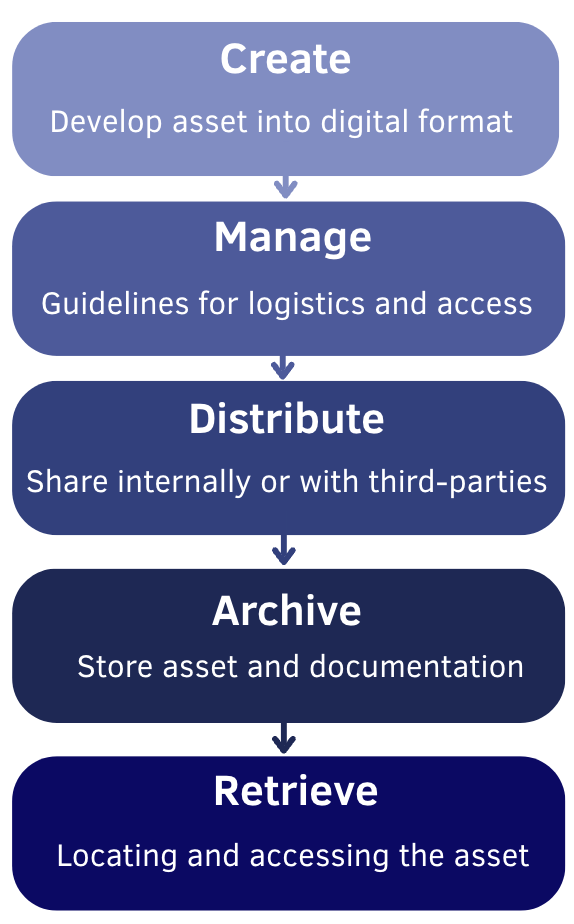
\includegraphics[width=0.5\linewidth]{4steg.png}  % Replace with actual image file
    \caption{Illustrating the five main stages of DAM.}
    \label{fig:4steg}  
\end{figure}

\vspace{0.3cm}
\subsubsection{Choosing a DAM and the key tasks}
\vspace{0.3cm}
What tools are available in DAM? 
Bechmark? 
What are the most important shit in it?
What do most companies need? 
What do they usually have and how or 
why do they choose to adopt a DAM

A missing perspective is 

\vspace{0.3cm}
\subsubsection{Technological Tools Demand Continuous Organizational Adaptation}
\vspace{0.3cm}

\cite{LOVE2019102930} identify a critical gap in the construction industry: knowing “why” 
to adopt digital technologies is relatively straightforward, but knowing “how” to translate 
technological potential into real value remains largely underexplored. Their case studies underscore 
the fact that digital transformation does not happen automatically; organizations must actively
 invest in processes such as benefits management and the development of a Business Dependency 
 Network (BDN) to realize tangible gains from their digital initiatives \citep{LOVE2019102930}.

 In a broader context, Hanelt et al. (2020) posit that digital transformation (DT) goes beyond 
any single disruptive episode; it is a continual, structural adjustment propelled by digital 
technologies. Their systematic review of 279 peer-reviewed articles frames DT across three 
dimensions—Contextual Conditions (e.g., technological advances, shifting consumer habits), 
Mechanisms (e.g., the innovative strategies organizations adopt), and Outcomes 
(e.g., changes to organizational structures and industry norms). By proposing 
a typology that spans technology impact, compartmentalized adaptation, systemic 
shift, and holistic co‐evolution, they challenge the idea of one-off change, 
advocating instead for an iterative, agile approach to transformation \citep{Haneltarticle}.

Taken together, these two perspectives highlight that while there is strong motivation to 
deploy new technologies (“why”), sustained, organization-wide benefits only materialize 
when there is a concerted effort to integrate, evaluate, and adapt these digital tools 
in an ongoing manner (“how”). Both studies imply that true success hinges on long-term 
structural and cultural shifts rather than static, one-off solutions.

\vspace{0.3cm}

that the promise of DAM
is not unlocked simply by adopting new technology but only when companies embrace two 
fundamental principles. First, that technology alone does not create value but must be accompanied by 
organizational process reengineering, and second, that the benefits of DAM 
are maximized only through continuous strategic governance to monitor and sustain its impact 


A missing perspective in

Nevertheless, some scholars argue that
resource possession alone does not guarantee successful 
digital transformation. 
\cite{Civelek2023} found no significant link be-
tween dynamic capabilities—a key aspect
of RBV that involves adapting, integrating,
and reconfiguring resources—and successful
digital transformation among Czech manu-
facturing SMEs. Their findings suggest that
merely possessing dynamic capabilities is
insufficient for digital transformation unless
supported by complementary factors such as
digital literacy and IT infrastructure matu-
rity.


\vspace{0.3cm}
\subsubsection{Why to make our own and not use a service}
\vspace{0.3cm}

% What about the benefits? A missing perspective in software engineering
% There are xxx characteristics that distinguish yyy from other information and communication
% technology (ICT) system, as shown in Figure 2-1. Table 2.1 summarizes these characteristics.

Bynder

% https://en.wikipedia.org/wiki/DBGallery

Adobe Experince Manager 

Cloudinary:  custom pricing for enterprise solutions.

Adobe sensei 
enerally means auto-tagging images based on recognizable 
generic objects, scenes, and concepts. It typically uses 
generalized, pre-trained models that identify common objects'

most DAM platforms rely on third-party integrations 
for company-specific tagging


Clarifai Custom Models
Provides APIs that integrate into DAM platforms.


Amazon Rekognition Custom Labels: Pay-per-use


Google Vertex AI (formerly AI Platform Vision)
Pricing depends on training hours and predictions
Custom vision API: Trained specifically on your images and product labels.

Microsoft Azure Custom Vision: Training: 20 dollaar per compute hour 

Integrates via REST API to enhance tagging accuracy in DAM solutions.

CV consutling 
% https://ventionteams.com/services/computer-vision

Image annotation 
% https://www.anolytics.ai/image-annotation-services/

Different types of CV:
% https://towardsdatascience.com/5-neural-network-architectures-you-must-know-for-computer-vision-31d2991fe24e/

\ref{fig:lit_review} is an image 
\ref{tab:lit_review} is a table

\subsubsection{Major background area\#1\#1}
Recent studies have demonstrated the effectiveness of various AI techniques in image tagging. 
Zhang et al. (2019) showcased the application of convolutional neural networks (CNNs) for automatic 
image classification in DAM systems, achieving an accuracy of 92\% on a diverse dataset of digital assets

This work was further extended by Li 
and Chen (2020), who integrated attention mechanisms into CNNs, improving the model's ability to focus on 
salient features and increasing tagging accuracy to 95\%

The YOLO (You Only Look Once) algorithm has also been applied successfully in DAM contexts. 
Wang et al. (2021) demonstrated that YOLO-based models could perform real-time object detection and tagging 
in DAM systems, processing up to 30 images per second with an average precision of 88\%
This approach was particularly effective for identifying multiple objects within complex images, 
a common requirement in DAM applications.

Transformer-based models have recently gained traction in image tagging for DAM systems. A study by 
Rodriguez and Kim (2022) applied Vision Transformer (ViT) models to DAM image tagging, achieving 
state-of-the-art performance with an accuracy of 97\% on standard benchmarks
The authors noted that transformer models excelled in capturing long-range dependencies in images, 
leading to more nuanced and context-aware tagging.


While AI-powered image tagging offers significant benefits, it also presents several challenges. Data requirements 
pose a significant hurdle, as highlighted by Brown et al. (2020), who found that AI models required at 
least 10,000 labeled images per category for optimal performance in domain-specific DAM applications

Error rates and handling domain-specific content remain ongoing challenges. A comprehensive study by 
Thompson et al. (2021) analyzed error patterns in AI-powered image tagging across various industries, 
revealing that error rates increased significantly (up to 25\%) when dealing with highly specialized or technical imagery

To address this issue, Nguyen and Patel (2022) proposed a hybrid approach combining pre-trained models with 
domain-specific fine-tuning, reducing error rates by 40\% in niche industries such as medical imaging and aerospace engineerin

Despite these challenges, the benefits of AI-powered image tagging in DAM systems are substantial. A large-scale study by Garcia et al. (2023)
 across 500 organizations found that implementing AI-powered tagging led to a 60\% reduction in manual tagging time and 
 a 35\% improvement in asset discoverability


Entangled states are an important part of quantum cryptography, but also relevant in other
domains. This concept might be relevant for neutrinos, see for example [2].

\paragraph{Scheme}



\subsubsection{The YOLO model}
\vspace{0.3cm}
As demonstrated in table \ref{tab:yolo_versions} the YOLO series has
 evolved significantly since its inception, introducing progressive improvements
  in object detection, computational efficiency, and feature extraction. 
YOLOv11 is the best choice for the project due to its superior accuracy, 
efficiency, and versatility. As Khanam and Hussain (2024) highlight, 
its architectural upgrades enhance feature extraction while minimizing 
computational costs, making it ideal for real-time applications requiring 
both speed and precision \citep{khanam2024yolov11overviewkeyarchitectural}.

\vspace{0.3cm}
Beyond object detection, YOLOv11 supports instance segmentation, 
pose estimation, and oriented object detection, offering greater adaptability 
to the project’s needs. Its optimized balance of accuracy and processing speed 
ensures strong performance across different computing environments, from edge 
devices to high-performance systems, making it the most effective solution





\begin{figure}[h]
    \centering
    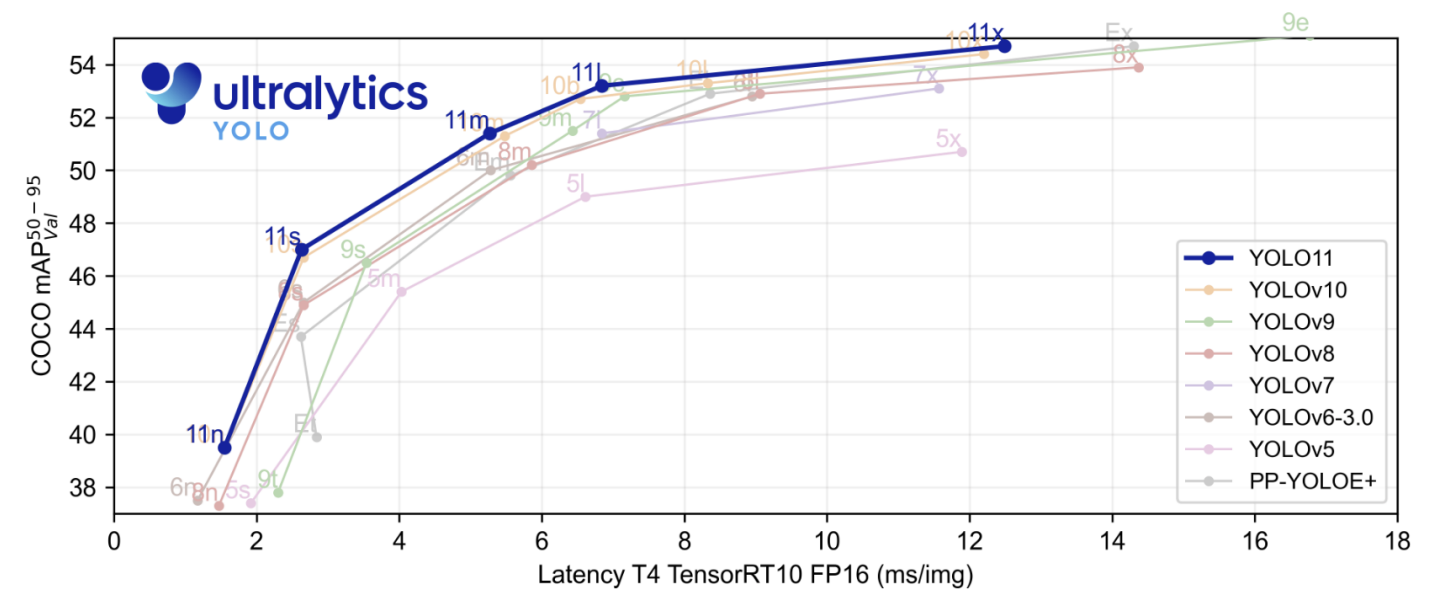
\includegraphics[width=1\linewidth]{YOLOV11.png}  % Replace with actual image file
    \caption{YOLOv11 performance comparison (Ultralytics Inc., 2025).}
    \label{fig:bench}  
\end{figure}

The selection of YOLOv11 for the project is driven by its superior architectural 
enhancements, versatile task support, and optimized balance between accuracy and 
efficiency. 
  Each version has incorporated refinements aimed at enhancing real-time performance, 
  with YOLOv11 representing the most advanced iteration to date \citep{khanam2024yolov11overviewkeyarchitectural}.
\vspace{0.3cm}


\subsection{Major background area\#2}
The application of AI-powered image tagging in DAM systems extends beyond large corporations 
to small and medium-sized enterprises (SMEs), particularly in premium manufacturing sectors. A case study 
by Hoffmann and Schulz (2022) examined the implementation of AI-powered DAM in a high-end carpentry 
company similar to Veermakers
The study found that AI-assisted tagging improved product catalog management 
efficiency by 45\% and reduced time-to-market for new designs by 30\%.

However, Chen et al. (2023) noted that SMEs in specialized manufacturing often 
face unique challenges in adopting AI-powered DAM systems, including limited datasets 
and highly specific visual content. 
To address these issues, the authors proposed a transfer learning approach, adapting pre-trained 
models to domain-specific tasks with minimal additional data, achieving a 75\% reduction in required 
training data while maintaining 90\% of the original accuracy.

While academic research has made significant strides in advancing AI-powered image tagging techniques, 
commercial implementations often lag behind in adopting cutting-edge methods. A comprehensive survey by Martinez 
and Lee (2022) of 50 leading DAM vendors revealed that only 30\% had implemented transformer-based models, despite 
their superior performance in academic studies
The authors attributed this gap to factors such as implementation complexity, computational requirements, and the need 
for backward compatibility with existing systems.




\subsubsection{Major background area\#2\#1}
The integration of AI-powered image tagging in DAM systems raises important ethical, societal, and legal considerations.
 Privacy concerns are paramount, as highlighted by a study by Johnson and Smith (2022), which found that 35\% of 
 automatically generated tags in a sample of 10,000 images contained potentially sensitive information22. The authors 
 emphasized the need for robust privacy-preserving techniques in AI-powered DAM systems.
 Algorithmic bias presents another significant challenge. Research by Park et al. (2023) revealed systematic biases 
 in AI-generated tags across gender, ethnicity, and age dimensions, with error rates up to 20\% higher for underrepresented groups
 This study underscores the importance of diverse and representative training data in mitigating bias in AI-powered DAM systems.
\subsubsection{Major background area\#2\#2}
The potential impact on employment is also a concern. While Garcia et al. (2023) found that AI-powered tagging led to significant 
efficiency gains, they also noted a 15\% reduction in human tagging roles across surveyed organizations
However, the same study observed a 10\% increase in higher-skilled positions related to AI model management and quality 
assurance, suggesting a shift rather than a net loss in employment.


\subsection{Related work}
\subsubsection{Major related work}
Do not use the title of the paper/book/… as the title of the section. Instead summarize what the contribution of this work is in your own words.

Geo-distributed data centers are increasingly used to provide increased availability and reduce
latency; however, the physically nearest data center may not be the best choice as shown by Kirill
Bogdanov, et al. in their paper “The Nearest Replica Can Be Farther Than You Think” [4].
Exploring decentralized approaches to AI model training, allowing organizations to collaborate on improving tagging accuracy while preserving data privacy.

\subsubsection{Major related work}
Carrier clouds have been suggested as a way to reduce the delay between the users and the cloud
server that is providing them with content. However, there is a question of how to find the available
resources in such a carrier cloud. One approach has been to disseminate resource information using
an extension to OSPF-TE, see Roozbeh, Sefidcon, and Maguire [5].

\subsubsection{Minor related work}
Do not use the title of the paper/book/… as the title of the section. Instead summarize what the contribution of this work is in your own words.

\subsection{Summary}
It is nice to bring this chapter to a close with a summary. For example, you might include a table that summarizes the ideas of others and the advantages and disadvantages of each – so that later you can compare your solution to each of these. This will also help guide you in defining the metrics that you will use for your evaluation.





% ===== Section 3: Methodology =====
\section{<Engineering-related content, Methodologies and Methods>
Use a self-explaining title}

The contents and structure of this chapter will change with your choice of methodology and methods.
For example, if you have implemented an artifact, what did you do and why? How will your evaluate it.


Describe the engineering-related contents (preferably with models) and the research methodology
and methods that are used in the degree project.
Give a theoretical description of the scientific or engineering methodology are you going to use
and why have you chosen this method. What other methods did you consider and why did you reject
them.
In this chapter, you describe what engineering-related and scientific skills you are going to
apply, such as modeling, analyzing, developing, and evaluating engineering-related and scientific
content. The choice of these methods should be appropriate for the problem. Additionally, you
should be consciousness of aspects relating to society and ethics (if applicable). The choices should
also reflect your goals and what you (or someone else) should be able to do as a result of your
solution - which could not be done well before you started.
The purpose of this chapter is to provide an overview of the research method used in this thesis.
Section 3.1 describes the research process. Section 3.2 details the research paradigm. Section 3.3
focuses on the data collection techniques used for this research. Section 3.4 describes the
experimental design. Section 3.5 explains the techniques used to evaluate the reliability and validity
of the data collected. Section 3.6 describes the method used for the data analysis. Finally, Section 3.7
describes the framework selected to evaluate xxx.

\subsection{Research Process}
Image of: steps conducted to do the research 
Fig: research processes


\subsection{Research Paradigm}

\subsection{Data Collection}
(This should also show that you are aware of the social and ethical concerns that might be relevant
to your data collection method.)

\subsubsection{Sampling}
1. Aa
2. Bb
3. Cc

\subsubsection{Sample Size}

\subsubsection{Target Population}


\subsection{Experimental design/Planned Measurements}


\subsubsection{Test environment/test bed/model}
Describe everything that someone else would need to reproduce your test environment/test
bed/model/…

\subsubsection{Hardware/Software to be used}


\subsection{Assessing reliability and validity of the data collected}

\subsubsection{Reliability}
How will you know if your results are reliable?

\subsection{Validity}
How will you know if your results are valid?



\subsection{Planned Data Analysis}

\subsubsection{Data Analysis Technique}
\subsubsection{Software Tools}


\subsection{Evaluation framework}




% ===== Section 4: WHAT has been Done =====
\section{[What you did – Choose your own chapter title to describe this]}
What have you done? How did you do it? What design decisions did you make? How did what you
did help you to meet your goals?

\subsection{Hardware/Software design …/ModelSimulation model parameters/…}
Figure 4-1 shows a simple icon for a home page. The time to access this page when served will be
quantified in a series of experiments. The configurations that have been tested in the test bed are
listed in Table 4-1.
\begin{figure}[htbp]
    \centering
    
\includegraphics[width=0.4\linewidth]{kthLogga.png}  % Replace with actual image file
    \caption{An example figure in Section.}
    \label{fig:ldone}  
\end{figure}

\begin{table}[htbp]
    \centering
    \begin{tabular}{|c|c|}
        \hline
        Column 1 & Column 2 \\
        \hline
        Data 1 & Data 2 \\
        Data 3 & Data 4 \\
        \hline
    \end{tabular}
    \caption{An example table in Section.}
    \label{tab:done}  
\end{table}



\ref{fig:ldone} is an image 
\ref{tab:done} is a table


\subsection{Implementation …/Modeling/Simulation/…}






% ===== Section 5: Results and analysis  =====
\section{Results and Analysis}
In this chapter, we present the results and discuss them.

Keep in mind: How you are going to evaluate what you have done? What are your metrics?
Analysis of your data and proposed solution
Does this meet the goals which you had when you started?

\subsection{Major results}
Some statistics of the delay measurements are shown in Table 5-1.
The delay has been computed from the time the GET request is received until the response is
sent.

\begin{table}[htbp]
    \centering
    \begin{tabular}{|c|c|}
        \hline
        Column 1 & Column 2 \\
        \hline
        Data 1 & Data 2 \\
        Data 3 & Data 4 \\
        \hline
    \end{tabular}
    \caption{An example table in Section}
    \label{tab:res}  
\end{table}

\ref{tab:res} is a table

\subsection{Reliability Analysis}
LALALA

\subsection{Validity Analysis}
LALALA


\subsection{Discussion}





% ===== Section 6: CONCLUSION  =====
\section{Conclusions and Future work}
<<Add text to introduce the subsections of this chapter.>>

\subsection{Conclusions}
Describe the conclusions (reflect on the whole introduction given in Chapter 1).
Discuss the positive effects and the drawbacks.
Describe the evaluation of the results of the degree project.
Did you meet your goals?
What insights have you gained?
What suggestions can you give to others working in this area?
If you had it to do again, what would you have done differently?

\subsection{Limitations}
What did you find that limited your efforts? What are the limitations of your results?

\subsection{Future work}
Describe valid future work that you or someone else could or should do.
Consider: What you have left undone? What are the next obvious things to be done? What hints
can you give to the next person who is going to follow up on your work?

\subsection{Reflections}
What are the relevant economic, social, environmental, and ethical aspects of your work?





% ===== Section 7: References =====

\addcontentsline{toc}{section}{References}  % Lägg till i innehållsförteckningen
\bibliographystyle{apalike}
\nocite{*}
\bibliography{references} % Hänvisar till din references.bib-fil


% \bibliographystyle{apalike}
% \nocite{*}
% \bibliography{references} % Ensure your references.bib file includes all cited sources




% ===== Appendices =====
\newpage
\onecolumn
\appendix  % This marks the start of the appendices
\phantomsection
\addcontentsline{toc}{section}{Appendices} % Adds "Appendices" to Table of Contents
\section*{Appendices} % Title for Appendices
\renewcommand{\thesubsection}{\Alph{subsection}} % Number subsections as A, B, C

\section{Appendix A: Example Appendix Title}
\label{appendix:A}
This is an example appendix entry. You can include figures, tables, or additional details relevant to your research.

\begin{figure}[htbp]
    \centering
    
\includegraphics[width=0.4\linewidth]{kthLogga.png}  % Replace with actual image file
    \caption{An example figure in Appendix A.}
    \label{fig:appendixA}  
\end{figure}

\begin{table}[htbp]
    \centering
    \begin{tabular}{|c|c|}
        \hline
        Column 1 & Column 2 \\
        \hline
        Data 1 & Data 2 \\
        Data 3 & Data 4 \\
        \hline
    \end{tabular}
    \caption{An example table in Appendix A.}
    \label{tab:appendixA}  
\end{table}

\newpage
\section{Appendix B: Another Appendix Example}
\label{appendix:B}
You can continue adding appendices in a similar manner.

IEEE Editorial Style Manual: 
	

\end{document}


